% vim: set textwidth=78 autoindent:

\section{Lavorare con dati OGC}

% when the revision of a section has been finalized, 
% comment out the following line:
%\updatedisclaimer

QGIS supporta sorgenti di dati WMS e WFS. Il supporto WMS è nativo, quello per
WFS è fornito tramite plugin.

\subsection{What is OGC Data}\index{OGC!introduction}

L'Open Geospatial Consortium (OGC), è un’organizzazione internazionale che raggruppa più
di 300 organizzazioni commerciali, governative, nonprofit e di ricerca.
I suoi membri sviluppano e implementano standards per contenuti e servizi geospaziali,
analisi GIS e scambio dati.

Dal Consorzio è stato quindi elaborato un numero crescente di specifiche per i modelli di
dati per garantire bisogni specifici riguardanti l'interoperabilità
nell'ambito della tecnologia geospaziale, inclusi i GIS. Ulteriori
informazioni all'indirizzo \url{http://www.opengeospatial.org/}.

Importanti specifiche OGC sono:

\begin{itemize}
\item \textbf{WMS} - Web Map Service
\item \textbf{WFS} - Web Feature Service
\item \textbf{WCS} - Web Coverage Service
\item \textbf{CAT} - Web Catalog Service
\item \textbf{SFS} - Simple Features for SQL
\item \textbf{GML} - Geography Markup Language
\end{itemize}

Ad oggi i servizi OGC-sono sempre più di uso comune per scambiare dati geografici fra
differenti implementazioni GIS. QGIS ora può gestire tre delle specifiche esposte sopra
tra cui SFS (tramite il supporto a PostgreSQL/PostGIS, vedi Sezione
\ref{label_postgis}); e WFS e WMS come client.


\subsection{Client WMS}\label{sec:ogc-wms}\index{WMS!client}\index{OGC!WMS!client}\index{rasters!WMS}

\subsubsection{Panoramica sul servizio WMS}\label{sec:ogc-wms-about}\index{WMS!client!about}

QGIS può agire come client WMS, nel rispetto delle specifiche 1.1, 1.1.1 e 1.3.
E’ stato particolarmente testato nei confronti di server accessibili pubblicamente
quali DEMIS e JPL OnEarth.

I server WMS rispondono alle richieste da parte dei clients (ad es. QGIS) di una mappa raster
di una determinata estensione, con un determinato insieme di strati, simboli e trasparenza.
Il server WMS quindi consulta le sue risorse (locali o remote), genera il raster e lo invia
al client in formato raster, per QGIS tipicamente come immagini JPEG o PNG.

WMS è un servizio REST (Representational State Transfer) piuttosto che un servizio web completo.
Come tale, si può prendere la URL (indirizzo del server con specifiche) generata da QGIS e usarla
in un browser web per ottenere la stessa immagine che QGIS usa internamente. Questo può essere
utile per identificare le cause di eventuali problemi, dato che esistono vari tipi di server
WMS e ciascuno ha la sua propria interpretazione degli standards WMS.

Gli strati WMS possono essere aggiunti molto semplicemente, una volta
disponibile l'indirizzo (URL) per accedere al server WMS, una connessione adatta
e posto che il server usi l’HTTP come meccanismo di trasferimento dati.

\subsubsection{Scegliere un server WMS}\label{sec:ogc-wms-servers}\index{WMS!remote server!selection}

La prima volta in cui si vuole utilizzare un servizio WMS, non sono presenti
server predefiniti. Si può avviare lo strumento cliccando sul pulsante
\toolbtntwo{mActionAddWmsLayer}{Aggiungi layer WNS} nella barra strumenti, 
oppure dalla voce di menù
\mainmenuopt{Layer}>\dropmenuopttwo{mActionAddWmsLayer}{Aggiungi layer WMS...}.
Si aprirà la finestra di dialogo \dialog{Aggiungi layer dal server}. È
possibile aggiungere alcuni servers cliccando sul pulsante
\button{Aggiungi server predefiniti}. Verranno quindi aggiunti almeno tre
servers WMS, incluso il server della NASA (JPL). Per definire un nuovo server WMS
nella sezione \tab{Connessioni server}, cliccare su \button{Nuovo} ed inserire
i parametri di connessione al server WMS desiderato, seguendo le indicazioni della
tabella \ref{tab:wms_connection_parms}:

\begin{table}[ht]\index{WMS!client!connection parameters}
\centering
\caption{Parametri del collegamento WMS}\label{tab:wms_connection_parms}\medskip
 \begin{tabular}{|l|p{5in}|}
\hline Nome & nome per la connessione che consenta di individuarlo nella
lista dei server WNS nel menù a tendina. \\
\hline URL \index{WMS!URL} &  indirizzo URL del server che fornisce i dati.
Deve essere un indirizzo raggiungibile, nello stesso formato che verrebbe
usato per aprire una connessione telnet o pingare un host. \\
\hline
\end{tabular}
\end{table}

È possibile, se necessario, impostare nelle opzioni i parametri del proxy per ricevere i servizi WMS da internet.
Selezionare la voce di menù \mainmenuopt{Impostazioni} >
\dropmenuopttwo{mActionOptions}{Opzioni} e cliccare sulla linguetta
\tab{Proxy}, nella quale è possibile inserire le impostazioni abilitando la
casella di controllo \checkbox{Utilizza un proxy per l'accesso web}.

Una volta creata la connessione al server WMS, essa sarà memorizzata e
disponibile per le successive sessioni di QGIS.

\begin{Tip}[ht]\caption{\textsc{A proposito di indirizzi dei server WMS}}
\qgistip{Quando si inserisce l'indirizzo del server URL, assicurarsi di
inserire l'indirizzo di base. Ad esempio non bisogna inserire frammenti tipo
\usertext{request=GetCapabilities} o \usertext{version=1.0.0} nell'indirizzo.\index{WMS!remote server!URL}
}
\end{Tip}

La tabella \ref{tab:wms_example_urls} mostra alcuni esempi di indirizzi di
server WMS con i quali iniziare.
Questi links sono stati controllati l'ultima volta nel Dicembre 2006, ma
potrebbere essere nel frattempo essere stati modificati:

%FIXME:  WMS URLs should be checked again and maybe extended in QGIS 

\begin{table}[ht]\index{WMS!remote server!URL!examples}
\centering
\caption{Esempi di indirizzi di server WMS pubblici}\label{tab:wms_example_urls}\medskip
 \begin{tabular}{|l|l|}
\hline \textbf{Name}        & \textbf{URL} \\
\hline Atlas of Canada      & http://atlas.gc.ca/cgi-bin/atlaswms\_en? \\
\hline DEMIS                & http://www2.demis.nl/wms/wms.asp?wms=WorldMap\& \\
\hline Geoscience Australia & http://www.ga.gov.au/bin/getmap.pl?dataset=national \\
\hline NASA JPL OnEarth     & http://wms.jpl.nasa.gov/wms.cgi? \\
\hline QGIS Users           & http://qgis.org/cgi-bin/mapserv?map=/var/www/maps/main.map\& \\
\hline
\end{tabular}
\end{table}

Un elenco esaustivi di servers WMS è reperibile all'indirizzo \url{http://wms-sites.com}.

\subsubsection{Caricare livelli WMS}\label{sec:ogc-wms-layers}\index{WMS!client!layers}

Una volta compilati correttamente i campi, si può premere sul pulsante
\button{Connetti} per ottenere le capacità del server. Tra queste sono inclusi
i formati immagine, i layer disponibili e i sistemi di proiezione forniti dal
server. Considerato che si tratta di operazioni in rete, la velocità nella
risposta dipenderà dalla qualità della connessione verso il server WMS. Mentre
si scaricano i dati dal server, l'avanzamento dell'operazione viene
visualizzato nella porzione inferiore sinistra della finestra. 

Lo schermo dovrebbe rassomigliare alla Figura \ref{fig:connection_wms}, che
mostra la risposta fornita dal server WMS NASA JPL OnEarth.

\begin{figure}[ht]
  \begin{center}
  	\caption{Finestra per l'aggiunta di un server WMS, nella quale vengono
	mostati gli strati disponibili \nixcaption}\label{fig:connection_wms}
	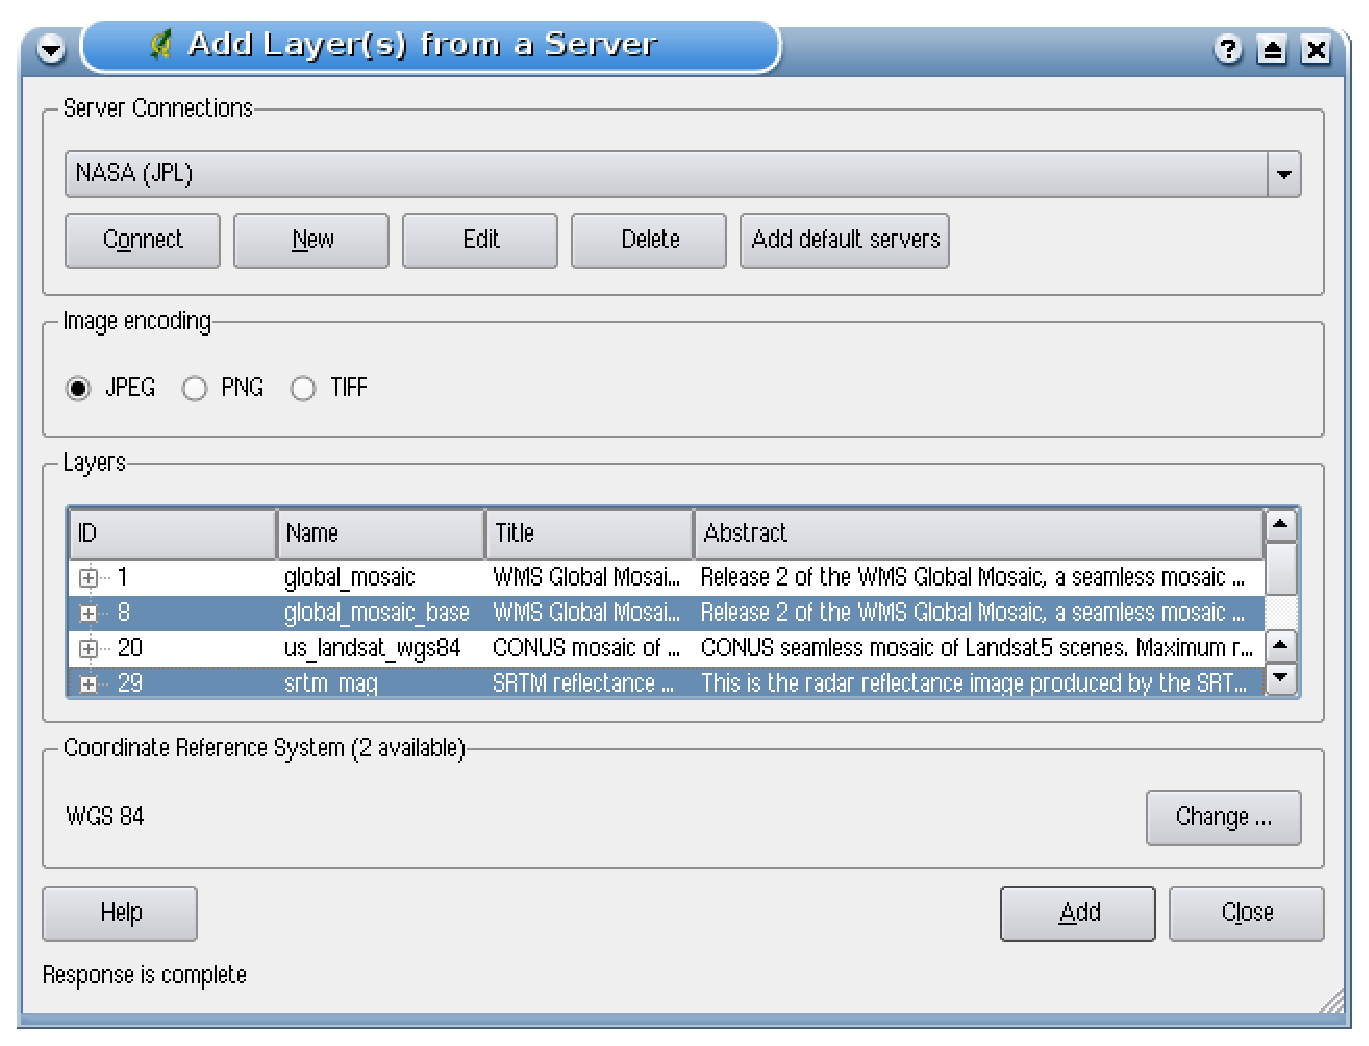
\includegraphics[clip=true,width=0.6\textwidth]{connection_wms}
  \end{center}
\end{figure}

\minisec{Codifica immagine}

La sezione \tab{Codifica immagine} elenca i formati supportati sia dal client
che dal  server. La scelta dipenderà dalla risoluzione che necessita allo scopo
prefisso.

\begin{Tip}[ht]\caption{\textsc{Codifica immagine}}
\qgistip{Solitamente un server WMS offrirà la scelta tra le codifiche JPEG e
PNG. Mentre la compressione JPEG comporta una perdita di qualità, quella PNG
riproduce fedelmente il dato di origine. Usare JPEG se non interessa avere una
certa perdita di qualità dell'immagine, riducendo d'altro canto il tempo per
il download dei dati di 5 volte rispetto al formato PNG. Usare invece PNG se
si vuole una rappresentazione precisa del dato originale e non ci si preoccupa
del tempo necessario per il trasferimento dei dati.
\index{WMS!image encoding}
}
\end{Tip}

\minisec{Layers}

La sezione \tab{Layer} elenca i livelli disponibili dal server WMS
selezionato. Si vedrà che alcuni layers sono espandibili, il che comporta che
essi possono essere mostrati in diversi stili di immagine.

Possono essere selezionati diversi layers alla volta, ma un solo stile di
immagine per ognuno di essi. Quando si effettua una selezione multipla, i
livelli vengono richiesti al server e trasmessi a QGIS in un solo blocco.

\begin{Tip}[ht]\caption{\textsc{Ordine degli strati WMS}}
\qgistip{In questa versione di QGIS, i layers WMS caricati sono sovrapposti in
base all'ordine in cui sono elencati nella sezione Layer, dall'alto verso il
basso. Se si desidera sovrapporre gli strati nel senso opposto occorre
selezionare una seconda volta \toolbtntwo{mActionAddWmsLayer}{Aggiungi layer
WMS}, scegliere nuovamente lo stesso server e selezionare il secondo gruppo di
strati che si desidera sovrapporre al primo.
\index{WMS!remote server!layer ordering}
}
\end{Tip}

\minisec{Trasparenza}\label{ogc-wms-transparency}

In questa versione di QGIS la trasparenza è impostata per essere sempre
attiva, se disponibile.

\begin{Tip}[ht]\caption{\textsc{Trasparenza dei Layer WMS}}
\qgistip{La possibilità di rendere trasparenti gli strati WMS dipenda dalla codifica tramite la quale sono stati caricati: PNG e GIF gestiscono la trasparenza mentre il JPEG no.
\index{WMS!layer transparency}
}
\end{Tip}

\minisec{Coordinate Reference System}
\index{WMS!CRS}\index{WMS!coordinate reference system}
\index{OGC!CRS}\index{OGC!coordinate reference system}
\index{Projections!WMS}
\index{Projections!CRS}\index{Projections!coordinate reference system}
\index{CRS}\index{coordinate reference system}
\index{SRS}\index{Projections!SRS}

A Coordinate Reference System (CRS) is the OGC terminology for a QGIS Projection.

Each WMS Layer can be presented in multiple CRSs, depending
on the capability of the WMS server.  You may notice that the \textsl{x} changes in
the \textsl{Coordinate Reference System (x available)} header as you
select and deselect layers from the \tab{Layers} section.

To choose a CRS, select \button{Change...} and a screen similar to
Figure \ref{fig:projections} in Section \ref{label_projstart} will appear.
The main difference with the WMS version of the screen is that only
those CRSs supported by the WMS Server will be shown.


\begin{Tip}[ht]\caption{\textsc{WMS Projections}}
\qgistip{For best results, make the WMS layer the first layer
you add in the project.  This allows the project
projection to inherit the CRS you used to render the WMS layer.
On-the-fly projection (see Section \ref{sec:projection-specifying})
can then be used to fit any subsequent
vector layers to the project projection.
In this version of QGIS, if you add a WMS layer later, and give it a different
CRS to the current project projection, unpredictable
results can occur.
}
\end{Tip}


\subsubsection{Using the Identify Tool}\label{sec:ogc-wms-identify}
\index{WMS!identify}
\index{identify!WMS}
\index{WMS!GetFeatureInfo}

Once you have added a WMS server, 
and if any layer from a WMS server is queryable, you can then use
the \toolbtntwo{mActionIdentify}{Identify} tool to select a pixel on the map canvas.
A query is made to the WMS server for each selection made.

The results of the query are returned in plain text.
The formatting of this text is dependent on the particular
WMS server used.

% FIXME: GetFeatureInfo-Requests are done here?

\subsubsection{Viewing Properties}\label{sec:ogc-wms-properties}\index{WMS!properties}
\index{rasters!properties}

Once you have added a WMS server, you can view its properties
by right-clicking on it in the legend, and selecting
\button{Properties}.


\minisec{Metadata Tab}\label{sec:ogc-wms-properties-metadata}
\index{rasters!metadata}
\index{WMS!metadata}
\index{WMS!capabilites}

The \tab{Metadata} tab displays a wealth of information about the WMS server,
generally collected from the Capabilities statement returned from
that server.

Many definitions can be gleaned by reading the WMS
standards \cite{OGCWMS010101web}, \cite{OGCWMS010300web}, but
here are a few handy definitions:

\begin{itemize}
\item \textbf{Server Properties}

\begin{itemize}
\item \textbf{WMS Version}      - The WMS version supported by the server.

\item \textbf{Image Formats}    - The list of MIME-types the server can respond with when
                                  drawing the map.  QGIS supports whatever formats
                                  the underlying Qt libraries were built with, which
                                  is typically at least \texttt{image/png} 
                                  and \texttt{image/jpeg}.

\item \textbf{Identity Formats} - The list of MIME-types the server can respond with when
                                  you use the Identify tool.  Currently QGIS supports
                                  the \texttt{text-plain} type.

\end{itemize}

\item \textbf{Layer Properties}

\begin{itemize}
\item \textbf{Selected}         - Whether or not this layer was selected when its                                                                        server was added to this project.

\item \textbf{Visible}          - Whether or not this layer is selected as visible
                                  in the legend.  (Not yet used in this version of QGIS.)

\item \textbf{Can Identify}     - Whether or not this layer will return any results
                                  when the Identify tool is used on it.

\item \textbf{Can be Transparent} - Whether or not this layer can be rendered with transparency.
                                    This version of 
                                    QGIS will always use transparency if this is \textsl{Yes}
                                    and the image encoding supports transparency
% BM: doesn't seem to work?
%                                    (see Section
%                                    \ref{ogc-wms-transparency}
%                                    ).
                                    .

\item \textbf{Can Zoom In}      - Whether or not this layer can be zoomed in by the server.  This version
                                  of QGIS assumes all WMS layers have this set to \textsl{Yes}.
                                  Deficient layers may be rendered strangely.

\item \textbf{Cascade Count}    - WMS servers can act as a proxy to other WMS servers to get
                                  the raster data for a layer.  This entry shows how
                                  many times the request for this layer is forwarded to peer
                                  WMS servers for a result.

\item \textbf{Fixed Width}, \textbf{Fixed Height}
                                - Whether or not this layer has fixed source pixel dimensions.
                                  This version
                                  of QGIS assumes all WMS layers have this set to nothing.
                                  Deficient layers may be rendered strangely.

\item \textbf{WGS 84 Bounding Box} - The bounding box of the layer, in WGS 84 coordinates.
                                     Some WMS servers do not set this correctly (e.g. UTM
                                     coordinates are used instead).  If this is the case,
                                     then the initial view of this layer may be rendered
                                     with a very ``zoomed-out'' appearance by QGIS.
                                     The WMS webmaster should be informed of this error,
                                     which they may know as the WMS XML elements
                                     \texttt{LatLonBoundingBox},
                                     \texttt{EX\_GeographicBoundingBox} or
                                     the CRS:84 \texttt{BoundingBox}.

\item \textbf{Available in CRS} - The projections that this layer can be rendered in by
                                  the WMS server.  These are listed in the WMS-native format.

\item \textbf{Available in style} - The image styles that this layer can be rendered in by
                                    the WMS server.

\end{itemize}

\end{itemize}


\subsubsection{WMS Client Limitations}\label{sec:ogc-wms-limits}\index{WMS!client!limits}

Not all possible WMS Client functionality had been included in this version of QGIS.
Some of the more notable exceptions follow:

\minisec{Editing WMS Layer Settings}
\index{WMS!layer settings!editing}

Once you've completed the \toolbtntwo{mActionAddWmsLayer}{Add WMS layer}
procedure, there is no ability to change the settings.

A workaround is to delete the layer completely and start again.

\minisec{WMS Servers Requiring Authentication}
\index{WMS!remote server!authentication}

Only public WMS servers are accessible.
There is no ability to apply a user name and password combination
as an authentication to the WMS server.

\begin{Tip}[ht]\caption{\textsc{Accessing secured OGC-layers}}
\qgistip{If you need to access secured layers, you could use InteProxy as
a transparent proxy, which does supports several authentification methods.
More information can be found at the InteProxy-manual found on the website
\url{http://inteproxy.wald.intevation.org}.
\index{WMS!secured layers!}\index{OGC!Authentication}
}
\end{Tip}


\subsection{WFS Client}

In QGIS, a WFS layer behaves pretty much like any other vector layer. You 
can identify and select features and view the attribute table. An exception 
is that editing is not supported at this time. To start the WFS plugin you 
need to open \mainmenuopt{Plugins} > \dropmenuopttwo{mActionShowPluginManager}{Plugin Manager...}, 
activate the \checkbox{WFS plugin} checkbox and click \button{OK}. 

A new \toolbtntwo{mIconAddWfsLayer}{Add WFS Layer} icon appears next 
to the WMS icon. Click on it to open the dialog. In General adding a WFS 
layer is very similar to the procedure used with WMS. The difference is 
there are no default servers defined, so we have to add our own.

\subsubsection{Loading a WFS Layer}

As an example we use the DM Solutions WFS server and display a layer. The URL is:
\begin{verbatim}
http://www2.dmsolutions.ca/cgi-bin/mswfs_gmap?VERSION=1.0.0&SERVICE=
wfs&REQUEST=GetCapabilities
\end{verbatim}

\begin{enumerate}
  \item Make sure the WFS plugin is loaded; if not, open the Plugin Manager and load it
  \item Click on the 
  \toolbtntwo{mIconAddWfsLayer}{Add WFS Layer} 
  tool on the plugins toolbar
  \item Click on \button{New} 
  \item Enter \inputtext{Name}{DM Solutions} as the name
  \item Enter the URL (see previous page)
  \item Click \button{OK} 
  \item Choose \selectstring{Server Connections}{DM Solutions} from the drop-down box
  \item Click \button{Connect} 
  \item Wait for the list of layers to be populated
  \item Click on the \clicklistitem{Canadian Land} layer
  \item Click \button{Add} to add the layer to the map
  \item Wait patiently for the features to appear
\end{enumerate}

\begin{figure}[ht]
  \begin{center}
  	\caption{Adding a WFS layer \nixcaption}\label{fig:wfs_dmsolutions}
	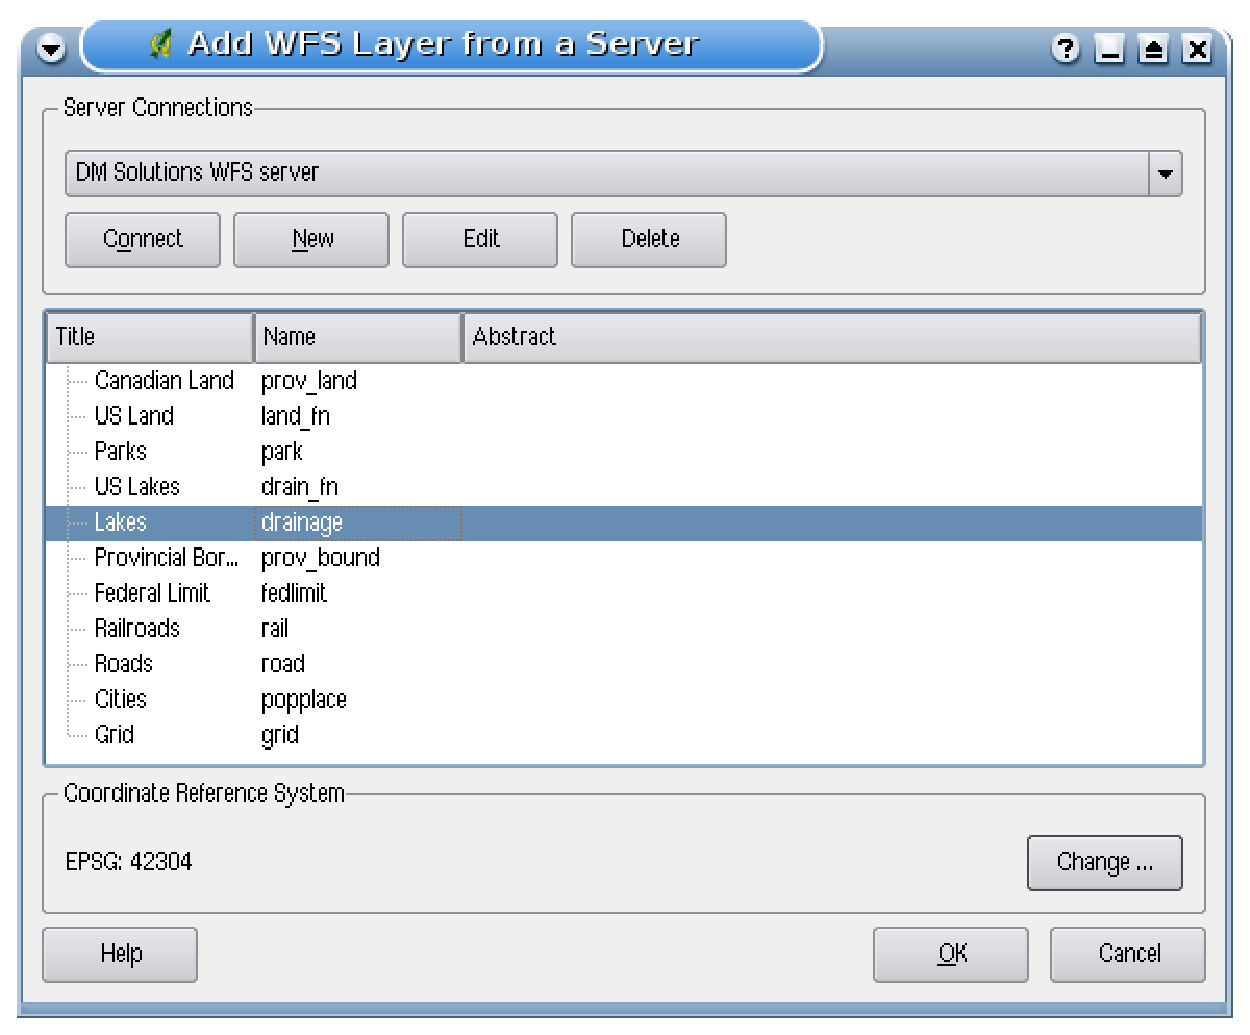
\includegraphics[clip=true,width=0.6\textwidth]{connection_wfs}
  \end{center}
\end{figure}

You'll notice the download progress is visualized in the left bottom of the QGIS main window. 
Once the layer is loaded, you can identify and select a province or two and view the 
attribute table.

Remember this plugin works best with UMN MapServer WFS servers. It still
could be, that you might experience random behavior 
and crashes. You can look forward to improvements in a future version of the plugin.

\begin{Tip}[ht]\caption{\textsc{Finding WMS and WFS Servers}}
\qgistip{You can find additional WMS and WFS servers by using Google or your
favorite search engine. There are a number of lists with public URLs, some 
of them maintained and some not.
\index{WFS!remote server!}
}
\end{Tip} 

